\documentclass[onecolumn, draftclsnofoot,10pt, compsoc]{IEEEtran}
\usepackage{graphicx}
\usepackage{url}
\usepackage{setspace}

\usepackage{geometry}
\geometry{textheight=9.5in, textwidth=7in}

% 1. Fill in these details
\def \CapstoneTeamName{Transportation Modeling}
\def \CapstoneTeamNumber{43}
\def \GroupMemberOne{Eytan Brodsky}
\def \GroupMemberTwo{Liang Du}
\def \GroupMemberThree{Samantha Estrada}
\def \GroupMemberFour{Shengjun Gu}
\def \GroupMemberFive{Charles Koll}
\def \CapstoneProjectName{Autonomous vehicle routing in congested transportation network.}
\def \CapstoneSponsorCompany{Oregon State University}
\def \CapstoneSponsorPerson{Haizhong Wang}

% 2. Uncomment the appropriate line below so that the document type works
\def \DocType{Requirements Document: Draft 2}

\newcommand{\NameSigPair}[1]{\par
\makebox[2.75in][r]{#1} \hfil 	\makebox[3.25in]{\makebox[2.25in]{\hrulefill} \hfill		\makebox[.75in]{\hrulefill}}
\par\vspace{-12pt} \textit{\tiny\noindent
\makebox[2.75in]{} \hfil		\makebox[3.25in]{\makebox[2.25in][r]{Signature} \hfill	\makebox[.75in][r]{Date}}}}
% 3. If the document is not to be signed, uncomment the RENEWcommand below
%\renewcommand{\NameSigPair}[1]{#1}

%%%%%%%%%%%%%%%%%%%%%%%%%%%%%%%%%%%%%%%
\begin{document}
\begin{titlepage}
    \pagenumbering{gobble}
    \begin{singlespace}
        %\includegraphics[height=4cm]{coe_v_spot1}
        \hfill
        % 4. If you have a logo, use this includegraphics command to put it on the coversheet.
        %\includegraphics[height=4cm]{CompanyLogo}
        \par\vspace{.2in}
        \centering
        \scshape{
            \huge CS Capstone \DocType \par
            {\large\today}\par
            \vspace{.5in}
            \textbf{\Huge\CapstoneProjectName}\par
            \vfill
            {\large Prepared for}\par
            \Huge \CapstoneSponsorCompany\par
            \vspace{5pt}
            {\Large\NameSigPair{\CapstoneSponsorPerson}\par}
            {\large Prepared by }\par
            Group\CapstoneTeamNumber\par
            % 5. comment out the line below this one if you do not wish to name your team
            \CapstoneTeamName\par
            \vspace{5pt}
            {\Large
                \NameSigPair{\GroupMemberOne}\par
                \NameSigPair{\GroupMemberTwo}\par
                \NameSigPair{\GroupMemberThree}\par
                \NameSigPair{\GroupMemberFour}\par
                \NameSigPair{\GroupMemberFive}\par
            }
            \vspace{20pt}
        }
        \begin{abstract}
        % 6. Fill in your abstract
            With the inclusion of autonomous vehicles into transportation network models, the method of how they will create optimal paths is questioned as well as how they will coexist with human driven vehicles.
            To address this issue, we intend to investigate the integration of connected autonomous vehicles (CAVs) and gain data suggesting that vehicle autonomy and the overall infrastructure of transportation may be restructured positively to include multiple intelligent agents.
            Additionally, this project will explore the impact of CAVs relative to transportation congestion, using a Python based framework and vehicle models to create data on how CAVs behave on a transportation network.
        \end{abstract}
    \end{singlespace}
\end{titlepage}
\newpage
\pagenumbering{arabic}
\tableofcontents
% 7. uncomment this (if applicable). Consider adding a page break.
%\listoffigures
%\listoftables
\clearpage

% 8. now you write!
\section{Introduction}
\subsection{System Purpose \& Scope}
The purpose of this project is to provide a framework and interface to simulate the behaviors of connected autonomous vehicles in a transportation network, represented as a grid network.
With this framework, models of autonomous vehicles will be created to participate in the simulation, allowing researchers to derive data on their contribution to traffic congestion.
\subsection{System Overview}
\subsubsection{System Context}
This system will be used in a research environment to observe autonomous vehicles and their behavior.
The data compiled from the simulations run on this system will be relevant to transportation infrastructure research and observation.
\subsubsection{System Functions}
This system will create a city transportation grid world to simulate autonomous and human driven vehicles on a Python based framework.
A simulation will be run by an input of vehicle data, including information such as what the vehicle’s type is, its acceleration, and whether it is autonomous or human driven.
Taking this data, a gridworld will be built, and vehicles will attempt to route to their destinations using a simple Dijkstra’s algorithm.
After a simulation is run, it will provide precise data for users, presenting a data for a given vehicle’s trajectory selected by the user.
The user may adjust the transportation system before each simulation, controlling the amount of CAV’s active and the number of vehicles overall.
This functionality is intended to be integrated with a GUI that will display the simulation in a playable and interactive format.
\subsubsection{User Characteristics}
Target users will be limited to researchers interested in transportation infrastructure, all able to navigate through the interface and understand the results of each simulation.
\subsection{Definitions}
\begin{itemize}
\item CAV - Connected Autonomous Vehicle.
\item HV - Human-driven Vehicle.
\item GUI - Graphical User Interface.
\item API - Application Programming Interface.
\end{itemize}
\section{References}
\begin{itemize}
\item Ying Liu, Lei Liu and Wei-Peng Chen. 2017. Intelligent Traffic Light Control Using Distributed Multi-agent Q Learning. arXiv:1711.10941v1 [cs.SY]
\item Rick Zhang, Federico Rossi and Marco Pavone. 2016. Routing Autonomous Vehicles in Congested Transportation Networks: Structural Properties and Coordination Algorithms. arXiv:1603.0093v2 [cs.MA]
\item Alireza Mostafizi, Mohammad Rayeedul Kalam Siam and Haizhong Wang, Ph.D. 2018.  Autonomous Vehicle Routing Optimization in a Competitive Environment: A Reinforcement Learning Application.
\end{itemize}
\section{System Requirements}
\subsection{Functional Requirements}
The project should give an accurate simulation of traffic under conditions specified by the user.
These conditions will be parts of a traffic environment such as infrastructure layout, vehicle types (connected autonomous vehicles and human-controlled vehicles), vehicle starting locations, and vehicle destinations.
The project should accurately simulate interactions between the environment and autonomous/human-controlled vehicles, taking into account factors such as acceleration, reaction time for human-controlled vehicles, traffic lights, and other traffic signs.
\subsection{Usability Requirements}
To make this a usable interface for testing traffic routing and simulation, we will need to develop an intuitive GUI.
Through this GUI, the user should be able to specify the number, position, and other parameters of variables in the environment.
These will include vehicles, road layouts, traffic signals, and speed limits.
The user should be able to simulate different conditions and pause the simulation at any time.
\subsection{Performance Requirements}
This system is required to be able to display to the user at a minimum of ten frames per second.
Each vehicle has an independent estimation about its optimal route.
By connections between vehicles, they will know conditions about roads around them.
This system will allow the user to add tens of thousands of vehicles into the testing environment.
All of these vehicles will have different destinations.
A metric to be used will be the average travel time of each agent.
\subsection{System Interface}
There will be a usable API in the server-side code.
It will include the vehicle destinations and location tracking.
In the system interface, there will be a few optional parameters that will be changeable by the user.
The user will be able to check the current status of each parameter:
\begin{itemize}
\item How much time will this route take
\item How far from the start point to the destination
\item How many intersections in the system
\end{itemize}
\subsection{System Modes and States}
The program will have a start state of an empty grid representing a transportation network, with which the user will begin their interaction.
From here, the user may manipulate the number or percentage of automated vehicles to the amount of human driven vehicles, along with beginning locations of each vehicle.
They may then enter the simulation state by pressing “start” or “run”.
The simulation will run, and then display a playback of what occurred.
The user will then be able to rerun the simulation with optionally different parameters.
\subsection{Environmental Conditions}
The program will run on Linux systems.
If there is enough time we can consider writing a version that works on Windows, but Linux makes it easier to run and test on available hardware.
We will use Python to edit program structure.
Then we will use JavaScript to visualize it.
We will separate the program into three files.
\subsection{System Security}
Security is not a major requirement for this project, since there are no network connections going outside of the local network.
Without access to the physical machine, there is no risk, and even with access to the local machine there is no sensitive information in the application.
\subsection{Information Management}
The user should be able to record and save simulations.
The user will have an option to save a simulation in some video format and a format unique to the application in order to load it into the user interface and make modifications to the simulation.
\subsection{System Life Cycle Sustainment}
The system will be developed until mid-March, at which point it will be in its useful phase.
Starting in June, unless a group decides to maintain the software, it will enter its legacy phase.
It will potentially be decommissioned if another group develops a more effective product.
\section{Gantt Chart}
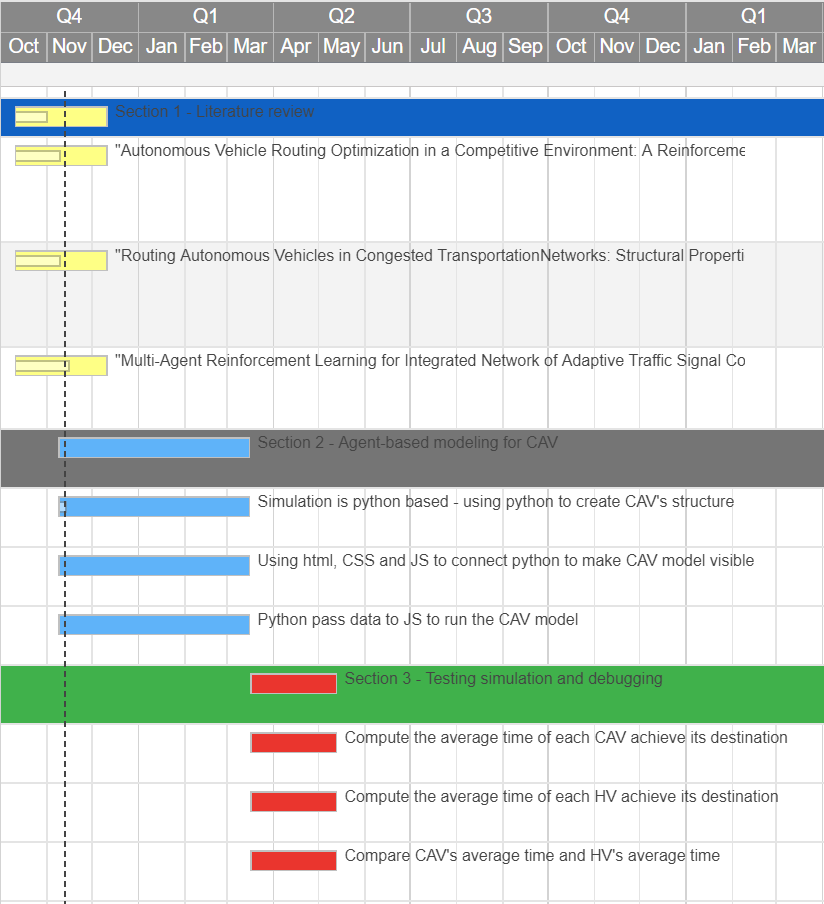
\includegraphics[width=5in]{gantt_chart}
\end{document}
